% ============================================================
% GenAI in the Everyday Worklife of an Actuary
% Minimal Beamer — VS Code Dark Modern / Light toggle
% ============================================================
\documentclass[aspectratio=169,10pt]{beamer}

% ── Dark / Light toggle ─────────────────────────────────────
% Set to true  → dark presentation (screen)
% Set to false → light presentation (print-friendly)
\newif\ifdarkmode
\darkmodetrue          % ← flip to \darkmodefalse for print
% ─────────────────────────────────────────────────────────────

\usepackage[T1]{fontenc}
\usepackage[utf8]{inputenc}
\usepackage{lmodern}
\usepackage{microtype}
\usepackage{hyperref}
\usepackage{xcolor}
\usepackage{tikz}
\usetikzlibrary{positioning, arrows.meta}
\usepackage{graphicx}
\graphicspath{{figures/}}
\usepackage{fontawesome5}        % icons (available on Overleaf)
\usepackage{enumitem}
\setlist[itemize]{label=\textcolor{accent}{\textbullet}}

% ── Colour palettes ─────────────────────────────────────────
\ifdarkmode
  % VS Code "Dark Modern"
  \definecolor{bg}{HTML}{1E1E1E}
  \definecolor{fg}{HTML}{D4D4D4}
  \definecolor{accent}{HTML}{007ACC}
  \definecolor{accentLight}{HTML}{569CD6}
  \definecolor{green}{HTML}{6A9955}
  \definecolor{orange}{HTML}{CE9178}
  \definecolor{yellow}{HTML}{DCDCAA}
  \definecolor{dimmed}{HTML}{808080}
  \definecolor{frameBorder}{HTML}{2D2D2D}
\else
  % Light counterpart (print-friendly)
  \definecolor{bg}{HTML}{FFFFFF}
  \definecolor{fg}{HTML}{1E1E1E}
  \definecolor{accent}{HTML}{005A9E}
  \definecolor{accentLight}{HTML}{0070C1}
  \definecolor{green}{HTML}{098658}
  \definecolor{orange}{HTML}{A31515}
  \definecolor{yellow}{HTML}{795E26}
  \definecolor{dimmed}{HTML}{6A6A6A}
  \definecolor{frameBorder}{HTML}{D4D4D4}
\fi

% ── Beamer chrome ────────────────────────────────────────────
\usetheme{default}
\usecolortheme{default}

\setbeamercolor{normal text}{fg=fg,bg=bg}
\setbeamercolor{structure}{fg=accent}
\setbeamercolor{alerted text}{fg=orange}
\setbeamercolor{frametitle}{fg=accentLight,bg=bg}
\setbeamercolor{title}{fg=accentLight,bg=bg}
\setbeamercolor{subtitle}{fg=dimmed}
\setbeamercolor{author}{fg=fg}
\setbeamercolor{date}{fg=dimmed}
\setbeamercolor{footer}{fg=dimmed,bg=bg}
\setbeamercolor{block title}{fg=bg,bg=accent}
\setbeamercolor{block body}{fg=fg,bg=frameBorder}
\setbeamercolor{itemize item}{fg=accent}
\setbeamercolor{itemize subitem}{fg=accentLight}

\setbeamerfont{title}{series=\bfseries,size=\Large}
\setbeamerfont{frametitle}{series=\bfseries,size=\large}

% suppress navigation symbols
\setbeamertemplate{navigation symbols}{}

% simple footline: short title | slide number
\setbeamertemplate{footline}{%
  \hspace{1em}%
  {\usebeamercolor[fg]{footer}\footnotesize
    \insertshorttitle\hfill\insertframenumber\,/\,\inserttotalframenumber}%
  \hspace{1em}\vskip4pt%
}

% Frame title with a thin accent rule
\setbeamertemplate{frametitle}{%
  \vskip6pt%
  {\usebeamerfont{frametitle}\usebeamercolor[fg]{frametitle}\insertframetitle}%
  \par\vskip-4pt%
  {\color{accent}\rule{\textwidth}{0.4pt}}%
  \vskip2pt%
}

% ── Meta ─────────────────────────────────────────────────────
\title{Generativ AI i aktuarens hverdag}
\subtitle{Praktiske anvendelseseksempler, læring og kognition}
\author{Anders Therkelsen}
\date{April 2026 \enspace · \enspace ASTIN}

% ─────────────────────────────────────────────────────────────
\begin{document}

% ── Title ────────────────────────────────────────────────────
{
\setbeamertemplate{footline}{}
\begin{frame}[plain,noframenumbering]
  \vfill
  \begin{center}
    {\usebeamerfont{title}\usebeamercolor[fg]{title}\inserttitle}\\[8pt]
    {\usebeamercolor[fg]{subtitle}\insertsubtitle}\\[16pt]
    {\usebeamercolor[fg]{author}\insertauthor}\\[4pt]
    {\usebeamercolor[fg]{date}\small\insertdate}
  \end{center}
  \vfill
\end{frame}
}

% ── Outline ──────────────────────────────────────────────────
\begin{frame}{Agenda}
  \begin{enumerate}[label=\textcolor{accent}{\arabic*.}]
    \item Foredragsholderens merit
    \item GenAI as a daily companion
    \item Concrete use-cases for actuaries
    \item Learning in the age of GenAI
    \item Cognitive caveats \& pitfalls
    \item Guidelines for responsible use
    \item Summary
  \end{enumerate}
\end{frame}

% ── Merit ────────────────────────────────────────────────
\begin{frame}{Foredragsholderens merit}
  \begin{columns}[T]
    % ── Left: bio bullets ──
    \begin{column}{0.55\textwidth}
      \begin{itemize}
        \item Anders Therkelsen, 35 år
        \item Oplært/opdraget af tre ledere:
          \begin{itemize}
            \item Helle Wicksell
            \item Jette Sandqvist
            \item Svend Haastrup
          \end{itemize}
        \item Far til Karl på 3 år og Frida på 5 måneder
        \item I branchen siden 2015
        \item Tidl. ASTIN-bestyrelsesmedlem, tidl.\\
              efteruddannelsesudvalget, bachelorvejleder
        \item Censor i matematik 2022--2026 og 2026--2030
      \end{itemize}
    \end{column}
    % ── Right: career timeline ──
    \begin{column}{0.42\textwidth}
      \vspace{0.3cm}
      \begin{tikzpicture}[%
          every node/.style={font=\normalsize},
          logo/.style={inner sep=0pt},
          cname/.style={text=fg, font=\normalsize, anchor=east},
          cyear/.style={text=dimmed, font=\normalsize, anchor=west},
        ]
        % All names have anchor=east → right edges at x=0
        % Arrow runs vertically at x=2pt (between name and year)
        \def\rowsep{1.5}

        % ── Row 1: Codan ──
        \node[cname] at (0, 0)          (c1name) {Codan};
        \node[cyear] at (4pt, 0)        (c1year) {(2015--2020)};
        \node[logo, right=6pt of c1year, anchor=west] (c1logo)
          {
\includegraphics[height=0.8cm]{codan_logo.png}};

        % ── Row 2: PwC ──
        \node[cname] at (0, -\rowsep)        (c2name) {PwC};
        \node[cyear] at (4pt, -\rowsep)      (c2year) {(2020--2023)};
        \node[logo, right=6pt of c2year, anchor=west] (c2logo)
          {
\includegraphics[height=0.8cm]{PwC_Company_Logo}};

        % ── Row 3: Alm Brand Group ──
        \node[cname] at (0, -2*\rowsep)      (c3name) {Alm Brand Group};
        \node[cyear] at (4pt, -2*\rowsep)    (c3year) {(2023--\ldots)};
        \node[logo, right=6pt of c3year, anchor=west] (c3logo)
          {
\includegraphics[height=0.8cm]{logo-alm-brand-group-rgb.png}};

        % ── Vertical arrows at x=2pt ──
        \draw[accent, thick, -{Stealth}]
          (2pt, -0.25) -- (2pt, -\rowsep+0.25);
        \draw[accent, thick, -{Stealth}]
          (2pt, -\rowsep-0.25) -- (2pt, -2*\rowsep+0.25);
      \end{tikzpicture}
    \end{column}
  \end{columns}
\end{frame}
% ── Section 1 ────────────────────────────────────────────────
\begin{frame}{GenAI as a Daily Companion}
  \begin{itemize}
    \item Large Language Models are \textcolor{accentLight}{general-purpose reasoning tools}
    \item Available 24/7 — low friction, high throughput
    \item Integration into IDEs, browsers, office suites
    \item Not a replacement for expertise; an \textcolor{green}{amplifier}
  \end{itemize}

  \vfill
  \begin{block}{Key principle}
    GenAI is most valuable when it meets domain knowledge halfway.
  \end{block}
\end{frame}

% ── Section 2 ────────────────────────────────────────────────
\begin{frame}{Use-Cases — Documentation \& Communication}
  \begin{itemize}
    \item \textcolor{yellow}{Drafting} technical documentation, model descriptions
    \item \textcolor{yellow}{Summarising} long regulatory texts, standards (e.g.\ IFRS\,17)
    \item \textcolor{yellow}{Translating} between audiences — board vs.\ regulator vs.\ IT
    \item Generating structured \textcolor{yellow}{templates} (reports, memos, slide decks)
  \end{itemize}

  \vspace{6pt}
  {\small\textcolor{dimmed}{%
    Tip: provide clear context \& constraints; iterate on the output.}}
\end{frame}

\begin{frame}{Use-Cases — Review \& Quality Assurance}
  \begin{itemize}
    \item Code review: spot bugs, suggest improvements, check style
    \item Spreadsheet auditing: formula consistency, edge-case testing
    \item Peer review of \textcolor{accentLight}{actuarial notes} — logic, clarity, completeness
    \item Cross-checking assumptions against published benchmarks
  \end{itemize}

  \vfill
  \begin{alertblock}{Caveat}
    GenAI can confidently produce plausible but \emph{wrong} output.\\
    Always verify numerical results independently.
  \end{alertblock}
\end{frame}

\begin{frame}{Use-Cases — Discussion \& Ideation}
  \begin{itemize}
    \item \textcolor{green}{Rubber-ducking}: explain a problem, get structured pushback
    \item Brainstorming model structures, risk factor hierarchies
    \item Exploring ``what if'' scenarios quickly
    \item Challenging your own reasoning — adversarial prompting
  \end{itemize}

  \vspace{6pt}
  {\small\textcolor{dimmed}{%
    Works best when you treat the model as a critical colleague,
    not an oracle.}}
\end{frame}

\begin{frame}{Use-Cases — Improving Own Work}
  \begin{itemize}
    \item Refactoring existing code (R, Python, VBA, SQL \ldots)
    \item Transforming ad-hoc scripts into \textcolor{accentLight}{reproducible pipelines}
    \item Generating unit tests, edge-case matrices
    \item Learning new libraries by example — ``show me how to \ldots''
  \end{itemize}
\end{frame}

% ── Section 3 ────────────────────────────────────────────────
\begin{frame}{Learning in the Age of GenAI}
  \begin{columns}[T]
    \begin{column}{0.48\textwidth}
      \textcolor{green}{\faThumbsUp}\enspace\textbf{Opportunities}
      \begin{itemize}
        \item Instant, personalised explanations
        \item Adaptive difficulty — Socratic mode
        \item Access to vast, cross-domain knowledge
        \item Faster feedback loops
      \end{itemize}
    \end{column}
    \begin{column}{0.48\textwidth}
      \textcolor{orange}{\faExclamationTriangle}\enspace\textbf{Risks}
      \begin{itemize}
        \item Illusion of understanding
        \item Reduced ``productive struggle''
        \item Shallow encoding → weak retention
        \item Over-reliance on generated answers
      \end{itemize}
    \end{column}
  \end{columns}
\end{frame}

% ── Section 4 ────────────────────────────────────────────────
\begin{frame}{Cognitive Caveats}
  \begin{enumerate}[label=\textcolor{accent}{\arabic*.}]
    \item \textbf{Automation bias} — trusting output because a machine said so
    \item \textbf{Cognitive offloading} — letting the tool think \emph{for} you
    \item \textbf{Skill atrophy} — ``use it or lose it'' applies to analytical rigour
    \item \textbf{Context collapse} — model lacks your institutional knowledge
    \item \textbf{Anchoring} — first AI-generated draft anchors subsequent thought
  \end{enumerate}

  \vfill
  {\small\textcolor{dimmed}{%
    These are not reasons to avoid GenAI — they are reasons to use it \emph{deliberately}.}}
\end{frame}

% ── Section 5 ────────────────────────────────────────────────
\begin{frame}{Guidelines for Responsible Use}
  \begin{itemize}
    \item \textbf{Verify} — never ship AI output without expert review
    \item \textbf{Understand} — if you cannot explain it, you do not own it
    \item \textbf{Alternate} — solve some problems \emph{without} AI to keep skills sharp
    \item \textbf{Prompt well} — invest time in clear, constrained prompts
    \item \textbf{Stay curious} — use AI to \textcolor{green}{deepen} understanding, not to skip it
  \end{itemize}

  \vfill
  \begin{block}{Rule of thumb}
    Use GenAI to \textbf{accelerate} what you already understand, and to
    \textbf{scaffold} what you are actively learning.
  \end{block}
\end{frame}

% ── Summary ──────────────────────────────────────────────────
\begin{frame}{Summary}
  \begin{center}
    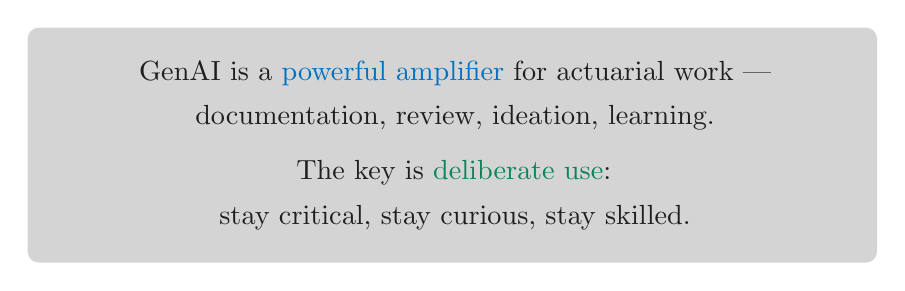
\begin{tikzpicture}
      \node[rounded corners=4pt, fill=frameBorder, text=fg,
            inner sep=12pt, text width=0.82\textwidth, align=center] {
        GenAI is a \textcolor{accentLight}{powerful amplifier} for actuarial work —\\[4pt]
        documentation, review, ideation, learning.\\[8pt]
        The key is \textcolor{green}{deliberate use}:\\[4pt]
        stay critical, stay curious, stay skilled.
      };
    \end{tikzpicture}
  \end{center}
\end{frame}

% ── Closing ──────────────────────────────────────────────────
{
\setbeamertemplate{footline}{}
\begin{frame}[plain,noframenumbering]
  \vfill
  \begin{center}
    {\Large\textcolor{accentLight}{Thank you}}\\[12pt]
    {\textcolor{dimmed}{Questions \& Discussion}}
  \end{center}
  \vfill
\end{frame}
}

\end{document}
